\documentclass[a4paper]{article}
\usepackage[T1]{fontenc}
\usepackage[utf8x]{inputenc}
\usepackage[italian,english]{babel}
\usepackage{amssymb,latexsym,amsfonts,amsmath}
\usepackage{lipsum}
\usepackage{url}
\usepackage{graphicx}
\usepackage[enable-survey]{pdfpages}

\begin{document}


\title{Esercitazione 5}
\date{April 5 , 2017}
\maketitle


\author{Alessio Susco \hspace*{2cm} Nicola Bomba \hspace*{2cm} Fabrizio Ursini  \\  \hspace*{1,85cm} Alessandra Di Martino \hspace*{1,25cm} Diego Guzman}

\includepdf[pages={1,2},pagecommand={\thispagestyle{plain}}]{eserc5.pdf} 

\tableofcontents

\clearpage


\section{Introduzione Generale}
Questa esercitazione è finalizzata alla verifica del funzionamento di alcuni componenti elettropneumatici e alla realizzazione di circuiti atti a svolgere diverse e specifiche funzioni.
L’esercitazione si struttura in quattro prove:
\begin{enumerate}
\item Verificare il funzionamento dei seguenti componenti elettropneumatici:
\begin{itemize}
\item valvola monostabile [comando diretto e comando indiretto (con relè];
\item valvola bistabile.
\end{itemize} 
\item Assemblare dei circuiti che realizzino le seguenti funzioni logiche:
\begin{itemize}
\item YES;
\item OR (diretto ed indiretto con relè);
\item AND (diretto ed indiretto con relè);
\item Autoaggancio.
\end{itemize} 
\item Realizzare due circuiti con attuatori pilotati da relè che realizzino i relativi diagrammi movimento-fasi;
\end{enumerate}


\section{Strumenti Utilizzati}

\subsection{Prova 1,2}

Banco dei relè, che comprende:
\begin{itemize}
\item Valvola monostabile a pulsante;
\item Valvola bistabile a leva;
\item Valvola monostabile a pulsante di emergenza;
\item Lampadine elettriche x2;
\item Lampadine pneumatiche x2;
\item Valvola monostabile a comando elettropneumatico;
\item Valvola bistabile a comando elettropneumatico;
\item Switch di accensione/spegnimento;
\item Relè x2;
\item Tubi in poliuretano;
\item Cavi elettrici;
\item Alimentazione pneumatica;
\item Alimentazione elettrica 24V.
\end{itemize}


\subsection{Prova 3}
Banco dei relè, che comprende:
\begin{itemize}
\item Valvola monostabile a pulsante;
\item Valvola bistabile a leva;
\item Valvola monostabile a pulsante di emergenza;
\item Lampadine elettriche x2;
\item Lampadine pneumatiche x2;
\item Valvola monostabile a comando elettropneumatico;
\item Valvola bistabile a comando elettropneumatico
\item Switch di accensione/spegnimento;
\item Relè x2
\item Tubi in poliuretano;
\item Cavi elettrici;
\item Alimentazione aria compressa;
\item Alimentazione elettrica 24V.
\end{itemize}

Banco degli attuatori, che comprende:
\begin{itemize}
\item Cilindri pneumatici a doppio effetto x3;
\item Valvole bistabili a comando elettropneumatico x3;
\item Valvole monostabili di fine corsa a comando elettropneumatico x6;
\item Tubi in poliuretano;
\item Cavi elettrici;
\item Alimentazione aria compressa;
\item Alimentazione elettrica 24V.
\end{itemize}


\section{Osservazione Preliminare}
\subsection{Prova 1}
Avvalendoci soltanto del banco dei relè, che comprende gli elementi elencati nella sezione “Strumenti utilizzati”, verifichiamo come prima istanza il funzionamento della valvola monostabile attraverso comando diretto e attraverso il relè, e ripetiamo lo stesso esperimento con la valvola bistabile. Costruiamo dei circuiti partendo dal collegamento dei cavetti elettrici che portano la corrente a tensioni 0-24V nella linea da dove in seguito collegheremo altri cavi che porteranno in tensione gli elementi elettropneumatici utili alla nostra prova (valvola monostabile a comando elettropneumatico e valvola bistabile a comando elettropneumatico). La prima parte viene svolta senza l’impiego dei relè, quindi colleghiamo direttamente l’alimentazione di aria compressa alle valvole e di seguito alle lampadine pneumatiche che ne constateranno le commutazioni quando si premono i pulsanti o si girano leve, che portiamo in tensione. Per la seconda parte della prova è necessario avvalersi dei relè, i quali portiamo in tensione con i cavi elettrici da 0 a 24V sulla linea NA. La presenza di corrente nella bobina è governata dal circuito di comando che formiamo partendo dal pulsante o dalla leva, che realizza le condizioni di attivazione delle due valvole elettropneumatiche.

\subsection{Prova 2}
Sullo stesso banco assembliamo dei circuiti che realizzino delle funzioni logiche. Per la realizzazione della funzione logica YES usiamo la valvola bistabile a leva. Quando c’è la presenza di comando tramite la leva la valvola viene commutata e l’aria compressa passa e accende la lampadina a sinistra o a destra dipendentemente dalla posizione della leva.
L'operatore logico OR si realizza collegando in parallelo più interruttori. In ambito elettrico due dispositivi si dicono in parallelo quando hanno in comune entrambi gli estremi di connessione. Nel nostro caso infatti colleghiamo in parallelo il pulsante alla valvola monostabile, per il caso del comando diretto. Per il comando indiretto tramite relè invece il collegamento in parallelo si effettua ai morsetti del comando della monostabile.
Nella connessione AND, l’operatore logico si realizza collegando in serie più interruttori. In ambito elettrico due dispositivi si dicono in serie quando hanno in comune solo uno degli estremi di connessione. La realizzazione è analoga al caso OR.
Infine per quanto riguarda l’autoaggancio, lo scopo principale dei circuiti in autoaggancio è di evitare la ripartenza automatica (rieccitazione della bobina) a seguito dell' interruzione dell' alimentazione. Quindi costruiamo il nostro circuito in modo che, per mezzo del pulsante viene chiuso e la bobina del relè, percorsa da corrente, crea un campo elettromagnetico destinato ad agire, in questo caso, su un ulteriore contatto. Infatti, oltre a comandare quello che governa il circuito esterno, opera su un secondo il quale si sposta in modo da garantire l'alimentazione alla bobina anche quando verrà rilasciato del pulsante di comando.

\subsection{Prova 3 e 4}
In questa prova e nella prossima ci viene assegnato un diagramma movimento fasi, quindi costruiamo un circuito usando il banco dei relè e quello degli attuatori.

\section{Schema Circuito}

\subsection{Esercizio 1.1 - Componenti Elettropneumatici}

\subsubsection{Valvola Monostabile}
\begin{center}
\includegraphics[scale=0.6]{circmonostabile.png}
\end{center}

\subsubsection{Valvola Bistabile}
\begin{center}
\includegraphics[scale=0.6]{circbistabile.png}
\end{center}


\section{Grafcet}

\subsection{Esercizio 1.3 - Attuatori pilotati da relè}
\begin{center}
\includegraphics[scale=0.6]{Grafcet1.png}
\end{center}

\subsection{Esercizio 2.3 - Attuatori pilotati da relè}
\begin{center}
\includegraphics[scale=0.6]{Grafcet2.png}
\end{center}

\section{Calcoli}
\dots

\section{Ladder Diagram}

\subsection{Esercizio 1.2 - Funzioni Logiche}

\subsubsection{YES}
\begin{center}
\includegraphics[scale=0.6]{laddermonostabile.png}
\end{center}

\subsubsection{AND}
\begin{center}
\includegraphics[scale=0.6]{ladderAND.png}
\end{center}

\subsubsection{OR}
\begin{center}
\includegraphics[scale=0.6]{ladderOR.png}
\end{center}

\subsubsection{Autoaggancio}
\begin{center}
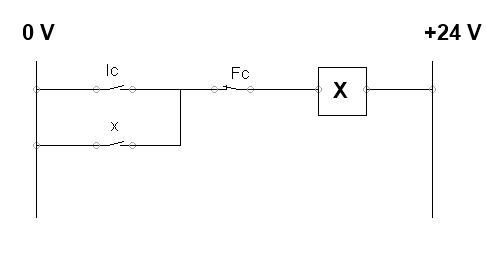
\includegraphics[scale=0.6]{Autoaggancio.png}
\end{center}


\subsection{Esercizio 1.3 - Attuatori pilotati da relè}
\begin{center}
\includegraphics[scale=0.6]{circLadder1.png}
\end{center}

\subsection{Esercizio 2.3 - Attuatori pilotati da relè}
\begin{center}
\includegraphics[scale=0.6]{circLadder2.png}
\end{center}

\section{Descrizione Approfondita dell'Esercitazione}
\subsection{Descrizione Esercizio 1}
...
\begin{itemize}
\item ...
\end{itemize}
...

\subsection{Descrizione Esercizio 2}
\dots

\section{Conclusioni}
\subsection{Conclusioni Esercizio 1}
\dots
\subsection{Conclusioni Esercizio 2}
\dots


\end{document}
